\section{Simulation Results}

To check that the calculations have been made correctly, an open loop simulation of the circuit was conducted. As it can be seen in figure \ref{fig:openloop_schematic} the circuit consists of the 4 MOSFETs, the inductor, the 2 capacitors and a load. The MOSFETs are controlled with two duty cycles D1 and D2. FET1 and FET4 will get the actual duty cycle while FET2 and FET3 uses the inverted duty cycles. With the scope the output voltage and current through the inductor can be visualized.

\begin{figure}[H]
	\begin{center}
		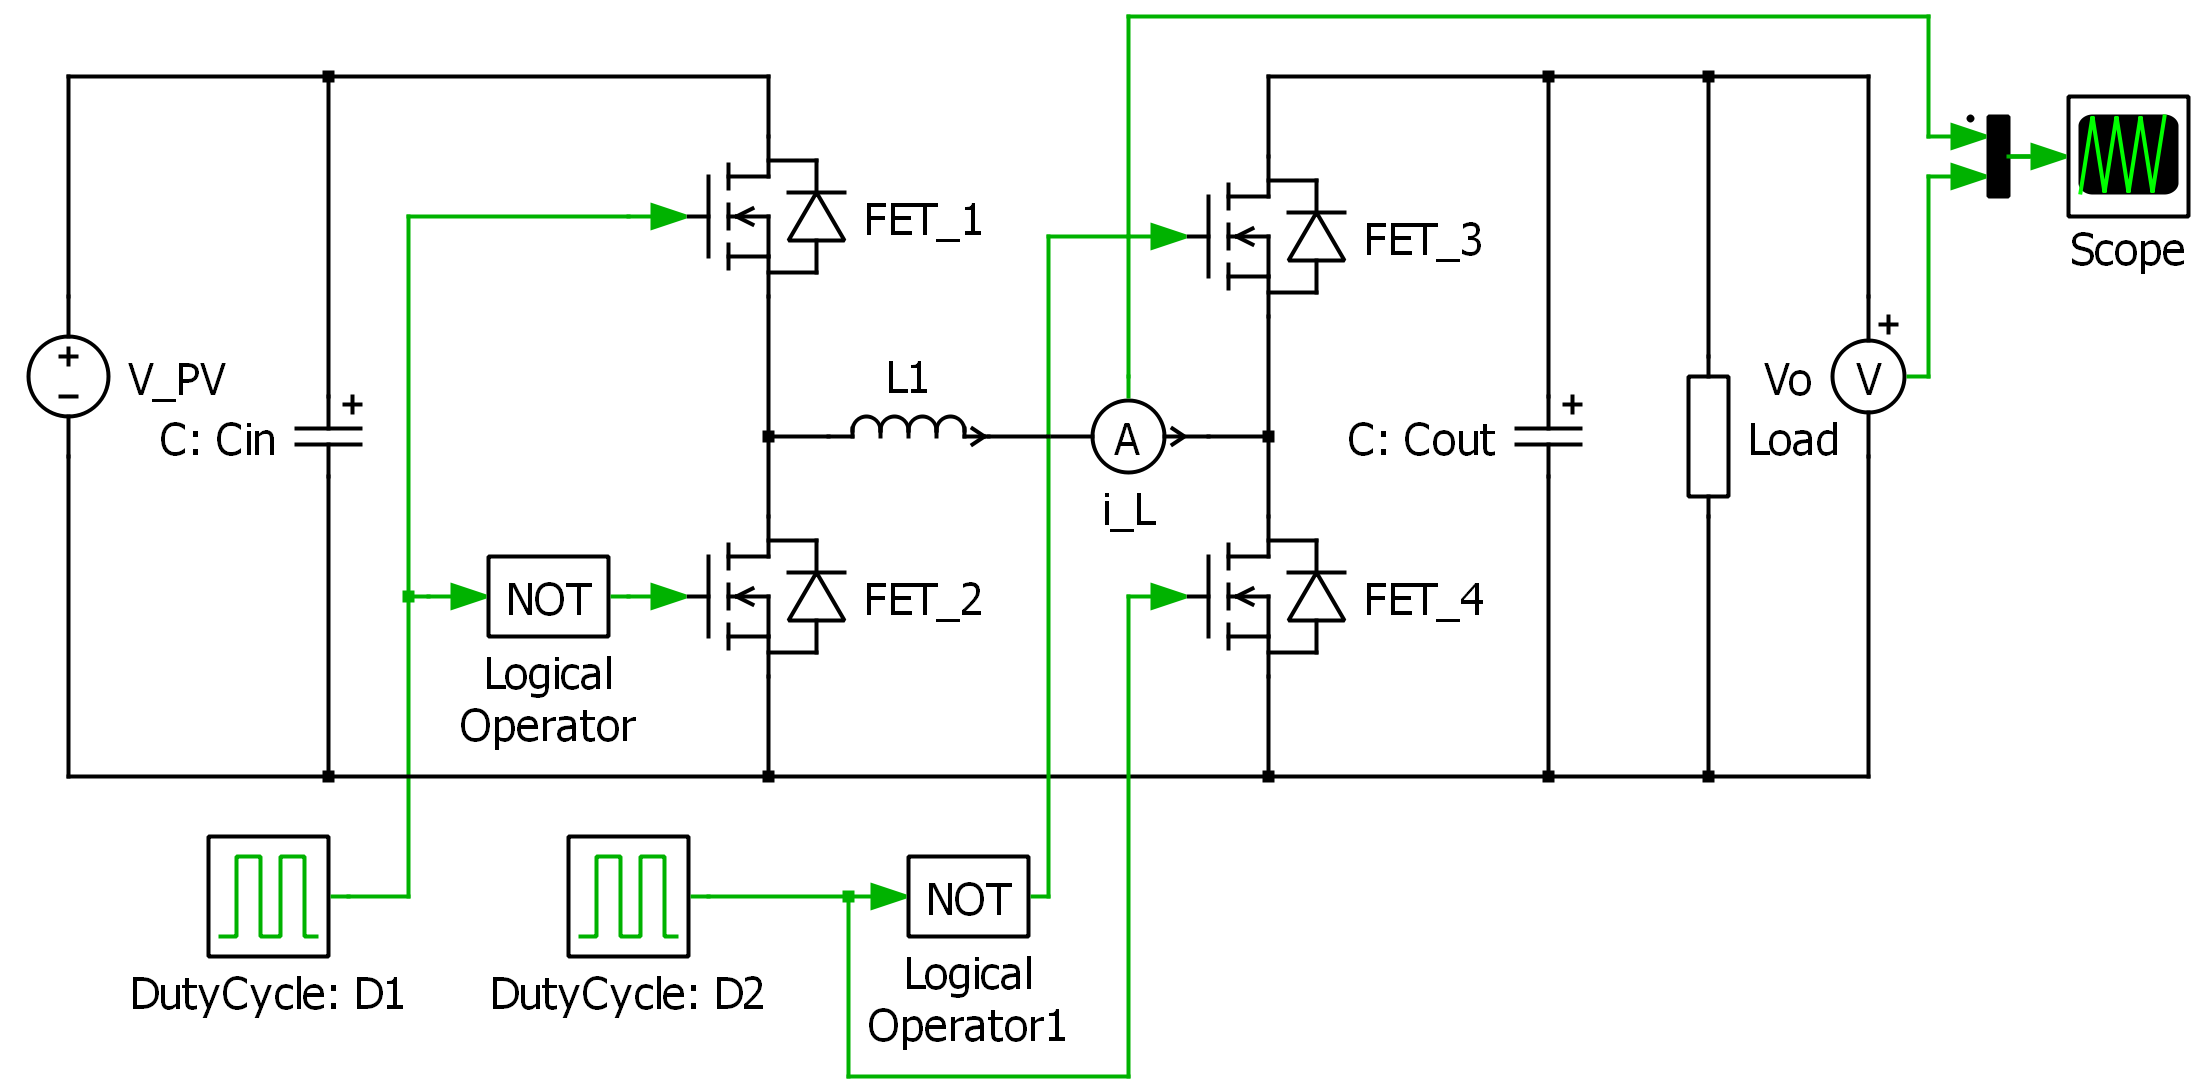
\includegraphics[width=0.7\textwidth]{../Pictures/P1/Open_loop_simulation/open_loop_schematic}
		\caption{Ideal open loop simulation}
		\label{fig:openloop_schematic}
	\end{center}
\end{figure}
The values for the components are $C_{in}=1880\mu F$, $C_{out}=820\mu F$ and $L1=1mH$ as described earlier and $V_{in}=36.9V$. At first the buck mode is simulated. In this mode D2 is 0. This means that FET4 is off and FET3 is on. The duty cycle for D1 is fixed at 0.65 which was calculated in \ref{buckduty}. This should give an output voltage of 24V which can be seen in figure \ref{bucksimulation}. The load is $1.92\Omega$ because it produces 300W with an output voltage at 24V.     
\begin{figure}[H]
 	\begin{center}
 		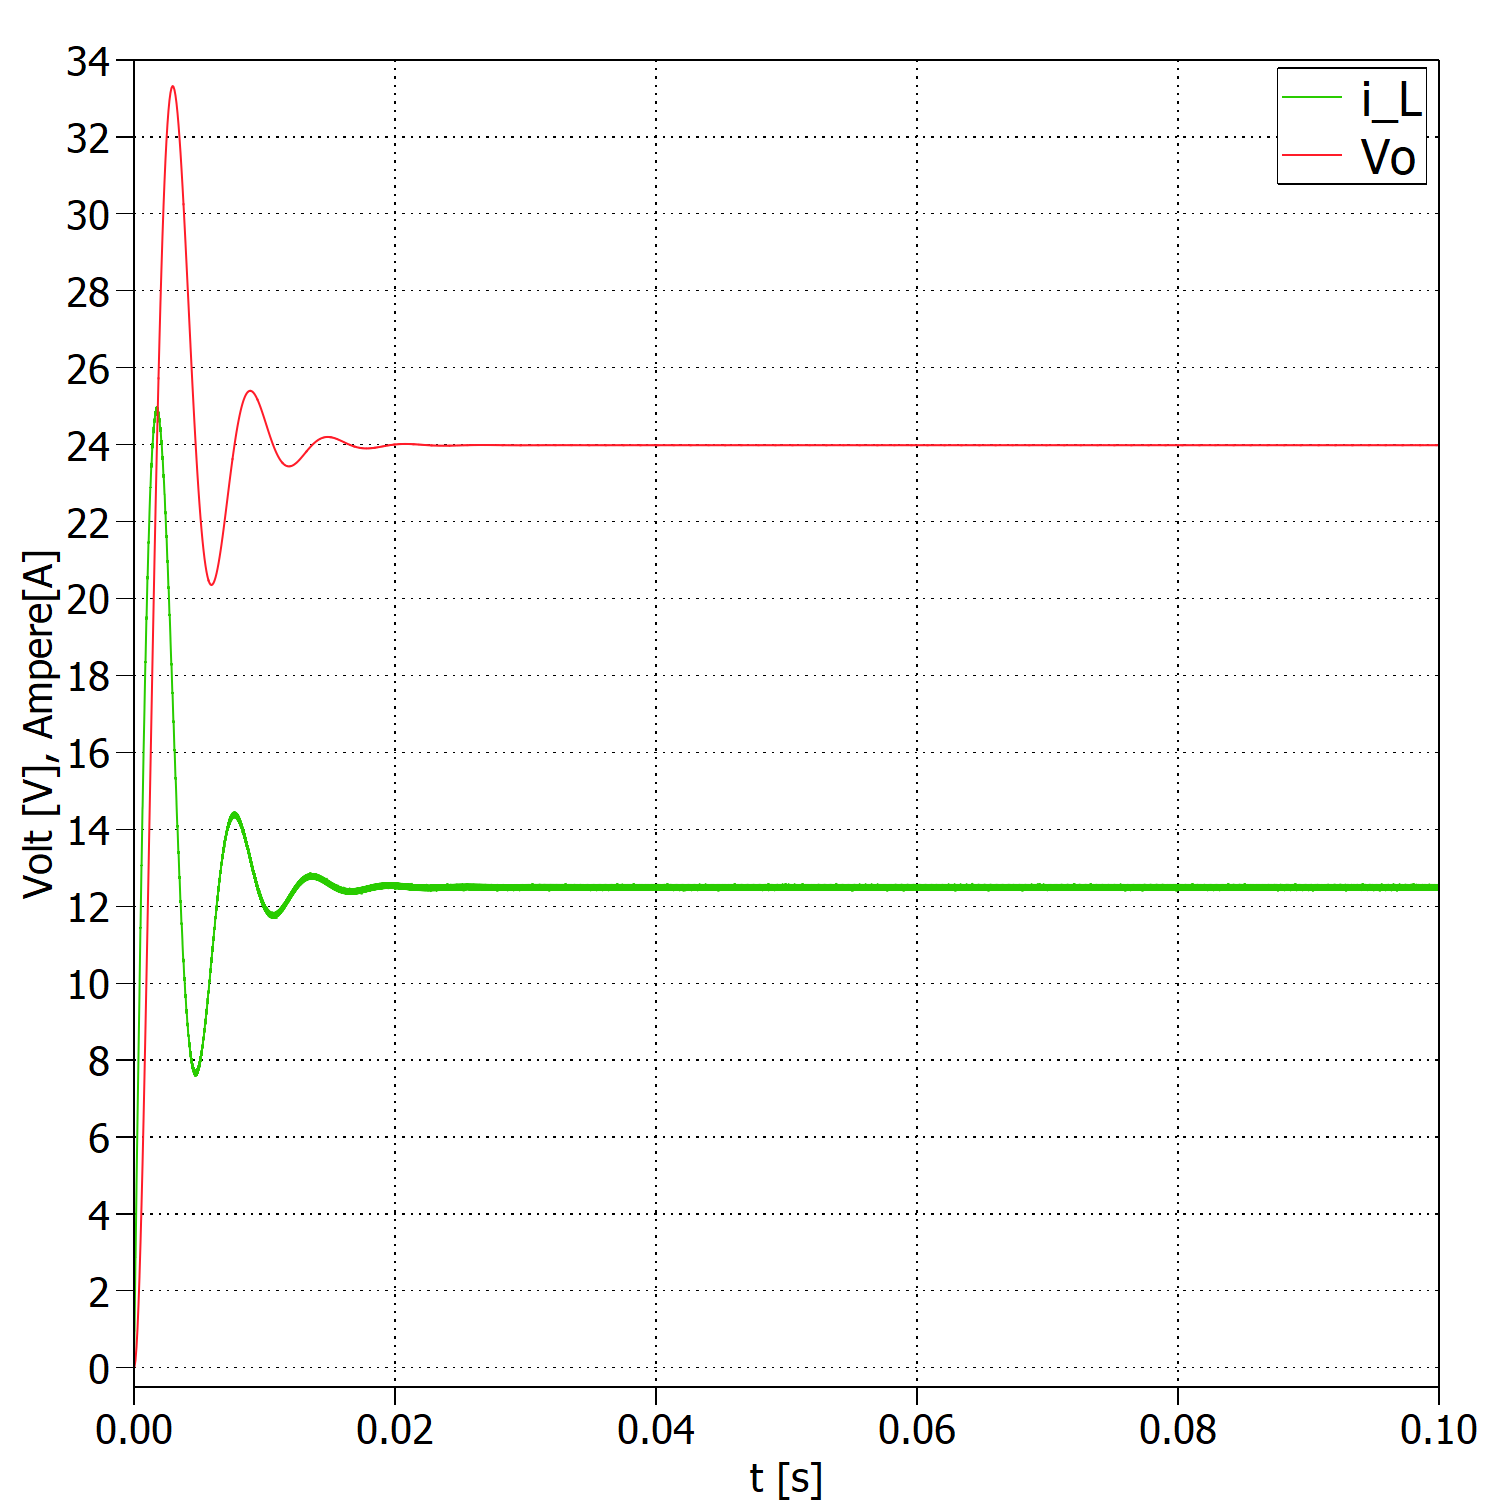
\includegraphics[width=0.5\textwidth]{../Pictures/P1/Open_loop_simulation/open_loop_buck}
 		\caption{open loop simulation of buck mode}
 		\label{bucksimulation}
 	\end{center}
\end{figure} 
In buck mode the current through the inductor should be equal to the output current \ref{iavg} which with a load of $1.92\Omega$ should be:
\begin{equation}
I_{out} = \frac{V_{out}}{R_{load}} = \frac{24V}{1.92\Omega} = 12.5A
\end{equation}   

To simulate the boost mode the input voltage is the same. Here the duty cycle for D2 is 0.638. This should correspond to an output voltage of 90V and calculated with the same equation as \ref{boostD}. D1 is fixed to 1 so that FET1 is on and FET2 is off. This should give an output voltage of 90V. With 90V the output current should be 9A and then the current through the inductor is calculated like this:

\begin{equation}
I_{L} = \frac{1}{1-0.638}\cdot 12.5A = 9.207A
\end{equation}  

In figure \ref{boostsim} steady state the red line is again the output voltage which is the expected 90V just as the green line which is the current through the inductor is a bit more than 9A.

\begin{figure}[H]
	\begin{center}
		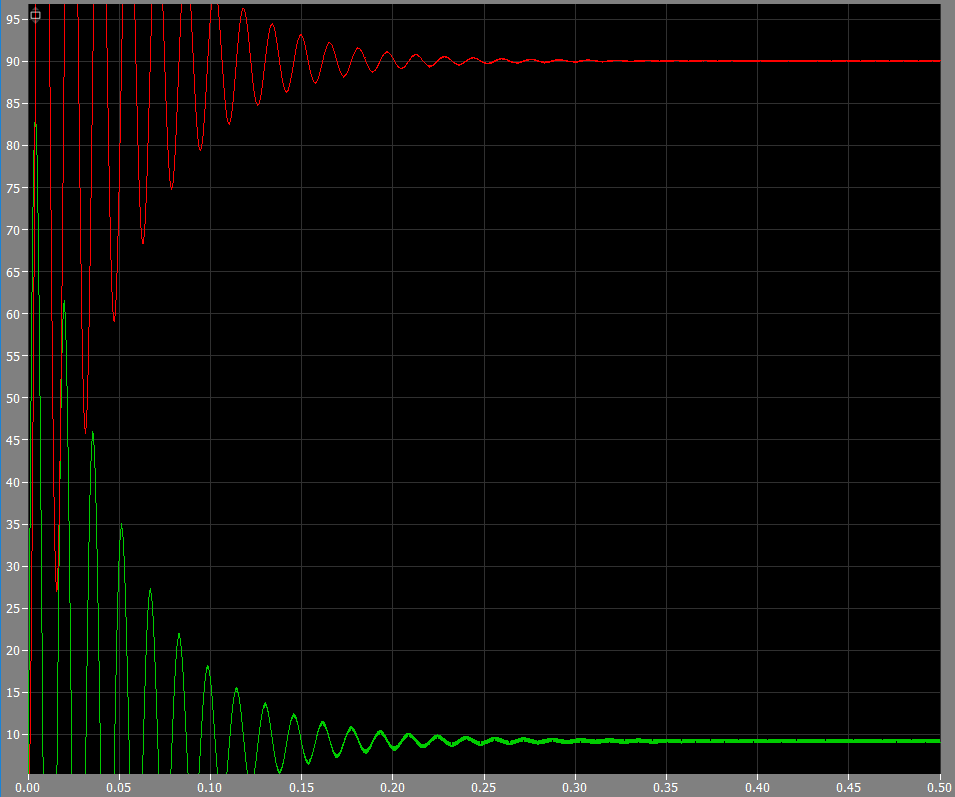
\includegraphics[width=0.5\textwidth]{../Pictures/boostsim}
		\caption{open loop simulation of boost mode}
		\label{boostsim}
	\end{center}
\end{figure}

\todo{This figure will be updated.}